%%%%%%%%%%%%%%%%%%%%%%%%%%%%%%%%%%%%%%%%%%%%%%%%%%%%%%%%%%%%%%%%%%%%%%%%%%%%%%%%%%%%%%%%%%%%%%%%%%%
%%%%%%%%%%%%%%%%%%%%%%%%%%%%%%%%%%%%%%%%%%%%%%%%%%%%%%%%%%%%%%%%%%%%%%%%%%%%%%%%%%%%%%%%%%%%%%%%%%%
%%%%%%%%%%%%%%%%%%%%%%%%%%%%%%%%%%%%%%%%%%%%%%%%%%%%%%%%%%%%%%%%%%%%%%%%%%%%%%%%%%%%%%%%%%%%%%%%%%%
%%%%%%%%%%%%%%%%%%%%%%%%%%%%%%%%%%%%%%%%%%%%%%%%%%%%%%%%%%%%%%%%%%%%%%%%%%%%%%%%%%%%%%%%%%%%%%%%%%%

\chapter{Metodolog\'ia}

El presente trabajo resulta de una colaboraci\'on con el departamento de Gerontolog\'ia, 
dependiente del Instituto de Ciencias de la Salud (ICSA).
Parte de esta colaboraci\'on incluye el acceso a los registros de PSG obtenidos por V\'azquez Tagle 
y colaboradores en 2016 \cite{VazquezTagle16}; por ello, se cita la metodolog\'ia de aqu\'el 
estudio de la manera m\'as fiel posible.
As\'i mismo se describe, a nivel de implementaci\'on, el an\'alisis central de este trabajo: la 
prueba de Priesltey-Subba Rao. 

%%%%%%%%%%%%%%%%%%%%%%%%%%%%%%%%%%%%%%%%%%%%%%%%%%%%%%%%%%%%%%%%%%%%%%%%%%%%%%%%%%%%%%%%%%%%%%%%%%%
%%%%%%%%%%%%%%%%%%%%%%%%%%%%%%%%%%%%%%%%%%%%%%%%%%%%%%%%%%%%%%%%%%%%%%%%%%%%%%%%%%%%%%%%%%%%%%%%%%%

\section{Participantes y su diagn\'ostico}

Los sujetos fueron elegidos usando un muestreo no probabil\'istico de sujetos tipo \cite{Garcia09},
firmando un consentimiento informado previamente a su inclusi\'on en el estudio. 
De manera extensiva, los criterios de exclusi\'on para el estudio fueron los siguientes:
\begin{itemize}
\item Firma del consentimiento informado
\item Edad entre 60 y 85 a\~nos
\item Diestros (mano derecha dominante)
\item Sin ansiedad, depresi\'on o s\'indromes focales
\item No usar medicamentos o sustancias para dormir
\item Voluntario para el registro de PSG
\end{itemize}

Un total de 9 participantes cumplieron todos los criterios de exclusi\'on y procedieron al registro 
de PSG; adicionalmente se tom\'o registro de otros tres adultos mayores, bajo
el consentimiento de \'estos y de los responsables del proyecto.

Usando los resultados obtenidos, los sujetos se dividieron en tres grupos:
\begin{description}
\item[Grupo PDC] (4 sujetos) Puntuaci\'on en Neuropsi menor a la media menos 3 desviaciones 
est\'andar, reportadas para poblaciones control \cite{Solis03}
\item[Grupo Control] (5 sujetos) Sin deterioro cognitivo
\item[Grupo Excluido] (3 sujetos) No satisfacen los criterios de inclusi\'on, pero que se 
sometieron voluntariamente al estudio con aprobaci\'on de los responsables
\end{description}

Con respecto al tercer grupo, se conforma de sujeto que fallan en exactamente uno de los criterios 
de inclusi\'on: FGH padece par\'alisis facial y posiblemente da\~no cerebral, MGG padece 
depresi\'on, y EMT no califica como adulto mayor por su edad.
Se efectuaron los mismos an\'alisis sobre este grupo con la finalidad de exhibir las capacidades y
limitaciones de las t\'ecnicas utilizadas, debido a lo cual este grupo es ignorado en la secci\'on 
de resultados, pero retomado en la discusi\'on.

\begin{table}
\centering
\bordes{1.1}
\begin{tabular}{c}
\textbf{Datos generales de los participantes}
\vspace{1em}
\end{tabular}
\begin{small}
\begin{tabular}{llcrrrrrrr}
\toprule
 \phantom{mm}&
 & \textbf{Sexo} & \textbf{Edad} & \textbf{Esc.} & \textbf{Neuropsi} & \textbf{MMSE} & \textbf{SATS} & \textbf{KATZ} & \textbf{Gds} \\
\midrule
\multicolumn{6}{l}{\textbf{Gpo. Control}}\\
&VCR    & F    & 59   & 12   & 107      & 29   & 21   & 0    & 3 \\
&MJH    & F    & 72   & 9    & 113      & 30   & 18   & 0    & 0 \\
&JAE    & F    & 78   & 5    & 102      & 28   & 19   & 0    & 5 \\
&GHA    & M    & 65   & 9    & 107.5    & 30   & 23   & 0    & 7 \\
&MFGR   & F    & 67   & 11   & 110      & 30   & 18   & 0    &   \\
\rowcolor{gris}
&\multicolumn{1}{c}{$\widehat{\mu}$} & 
              & 68.20& 9.20 & 107.90   & 29.40& 19.80& 0.00 & 3.00\\
\rowcolor{gris}
&\multicolumn{1}{c}{$\widehat{\sigma}$} & 
              & 7.19 & 2.68 & 4.07     & 0.89 & 2.17 & 0.00 & 3.08\\
\midrulec
%\hline
\multicolumn{6}{l}{\textbf{Gpo. PDC}}\\
&CLO    & F    & 68   & 5    & 81       & 28   & 22   & 1    & 6 \\
&RLO    & F    & 63   & 9    & 90       & 29   & 20   & 0    & 3 \\
&RRU    & M    & 69   & 9    & 85       & 27   & 10   & 0    & 3 \\
&JGZ    & M    & 65   & 11   & 87       & 25   & 20   & 0    & 1 \\
\rowcolor{gris}
&\multicolumn{1}{c}{$\widehat{\mu}$} & 
              & 66.25& 8.50 & 85.75   & 27.25& 18.00& 0.25 & 3.25\\
\rowcolor{gris}
&\multicolumn{1}{c}{$\widehat{\sigma}$} & 
              & 2.75 & 2.52 & 3.77    & 1.71 & 5.42 & 0.50 & 2.06\\
\midrule
%\hline
\multicolumn{6}{l}{\textbf{Sujetos excluidos}}\\
&FGH    & M    & 71   & 9    & 83.5     & 21   & 23   & 0    & 4  \\
&MGG    & F    & 61   & 9    & 114      & 28   & 29   & 1    & 14 \\
&EMT    & M    & 50   & 22   & 106      & 30   & 15   & 0    & 4  \\
\bottomrule
\end{tabular} 
\end{small}
\label{tab_sujetos}
\caption{Resultados de las pruebas neuropsicol\'ogicas aplicadas a los sujetos considerados en este 
trabajo, adem\'as de algunos datos generales. 
}
\end{table}

%%%%%%%%%%%%%%%%%%%%%%%%%%%%%%%%%%%%%%%%%%%%%%%%%%%%%%%%%%%%%%%%%%%%%%%%%%%%%%%%%%%%%%%%%%%%%%%%%%%
%%%%%%%%%%%%%%%%%%%%%%%%%%%%%%%%%%%%%%%%%%%%%%%%%%%%%%%%%%%%%%%%%%%%%%%%%%%%%%%%%%%%%%%%%%%%%%%%%%%

\section{Registro del polisomnograma}

Los adultos mayores participantes fueron invitados a acudir a las instalaciones de la Cl\'inica 
Gerontol\'ogica de Sue\~no (ubicadas dentro del Instituto de Ciencias de la Salud) para llevar a 
cabo el registro. Los participantes recibieron instrucciones de realizar una rutina normal de 
actividades durante la semana que precedi\'o al estudio, y se les recomend\'o que no ingirieran 
bebidas alcoh\'olicas o energizantes (como caf\'e o refresco) durante las 24 horas previas al 
experimento, ni durmieran siesta ese d\'ia.

El protocolo de PSG incluye 19 electrodos de EEG, 4 electrodos de EOG para registrar movimientos 
oculares horizontales y verticales, y 2 electrodos de EMG colocados en los m\'usculos 
submentonianos para registrar la actividad muscular. 
La colocaci\'on de los electrodos para registrar la actividad EEG se realiz\'o siguiendo las 
coordenadas del Sistema Internacional 10-20\cite{Coleman87}.

Debido a problemas t\'ecnicos con el electroencefal\'ografo, el registro se llev\'o a cabo a 512 Hz 
para algunos sujetos y a 200 Hz para otros; la recomendaci\'on de la AASM, de un m\'inimo de 128 
Hz, se satisface. 
Las se\~nales fueron amplificadas (amplificador de alta ganancia en cadena), filtradas (filtro paso 
de banda de 0.5--30 Hz) y digitalizadas para su posterior an\'alisis.
En la tabla \ref{frecuencias} se reportan la duraci\'on de estos registros para cada sujeto.

\begin{table}
\centering
\bordes{1.2}
\begin{tabular}{c}
\textbf{Datos generales sobre los registros de PSG}
\vspace{1em}
\end{tabular}
\begin{tabular}{llcrrcrrr}
\toprule
    \phantom{mm}&
    &\multirow{2}{*}{\begin{tabular}{c}\bordes{1}Frecuencia\\ muestreo\end{tabular}}
    \bordes{1.2}
    & \multicolumn{2}{c}{Total} & \phantom{l}   & \multicolumn{3}{c}{MOR}\\
    \cmidrule{4-5}  \cmidrule{7-9}
    &&          &Puntos  &  Tiempo   &&Puntos  &  Tiempo   &  \% MOR \\
\midrule
\multicolumn{6}{l}{\textbf{Gpo. Control}}\\
&VCR &200       & 5166000&   7:10:30 &&438000  &   0:36:30 & 8\% \\
&MJH &512       &15851520&   8:36:00 &&1950720 &   1:03:30 &12\% \\
&JAE &512       &13931520&   7:33:30 &&2626560 &   1:25:30 &19\% \\
&GHA &200       &6558000 &   9:06:00 &&330000  &   0:27:30 & 5\% \\
&MFGR&200       &4932000 &   6:51:00 &&570000  &   0:47:30 &12\% \\

\midrule

\rowcolor{gris}
\multicolumn{9}{l}{\textbf{Gpo. PDC}}\\
\rowcolor{gris}
&CLO &512       &14499840&   7:52:00 &&2027520 &   1:06:00 &14\% \\
\rowcolor{gris}
&RLO &512       &12994560&   7:03:00 &&1520640 &   0:49:30 &12\% \\
\rowcolor{gris}
&RRU &200       &2484000 &   3:27:00 &&228000  &   0:19:00 & 9\% \\
\rowcolor{gris}
&JGZ &512       &18539520&  10:03:30 &&506880  &   0:16:30 & 3\% \\

\midrule

\multicolumn{6}{l}{\textbf{Sujetos excluidos}}\\
&FGH &512       &6220800 &   3:22:30 &&337920  &   0:11:00 & 5\% \\
&MGG &512       &15820800&   8:35:00 &&2549760 &   1:23:00 &16\% \\
&EMT &512       &21857280&  11:51:30 &&721920  &   0:23:30 & 3\% \\
\bottomrule
\end{tabular}
\caption{Cantidad de datos analizados para cada sujeto. Debido a un cambio en el polisomn\'ografo 
usado, la frecuencia de muestreo (en Hz) cambia entre sujetos.
Dado que el sue\~no MOR aparece fragmentado, se reporta la suma de esos tiempos.}
\label{frecuencias}
\end{table}

La clasificaci\'on de las diferentes fases del sue\~no en el registro PSG se realiz\'o manualmente 
sobre \'epocas de EEG de 30 segundos siguiendo los criterios 
estandarizados de la AAMS\cite{Hori01}, mismas que fueron descritas anteriormente.

%%%%%%%%%%%%%%%%%%%%%%%%%%%%%%%%%%%%%%%%%%%%%%%%%%%%%%%%%%%%%%%%%%%%%%%%%%%%%%%%%%%%%%%%%%%%%%%%%%%
%%%%%%%%%%%%%%%%%%%%%%%%%%%%%%%%%%%%%%%%%%%%%%%%%%%%%%%%%%%%%%%%%%%%%%%%%%%%%%%%%%%%%%%%%%%%%%%%%%%

\section{Aplicaci\'on de la prueba PSR}

Los registros digitalizados de PSG fueron convertidos a formato de texto bajo la codificaci\'on 
ASCII, a raz\'on de un archivo por cada canal. 
Las \'epocas MOR fueron se\~naladas en archivos a parte, uno por cada sujeto.

Como se mencion\'o en secciones anteriores, la prueba PSR est\'a pensada para series de tiempo con 
media 0, varianza finita y espectro puramente continuo. Se espera que la segunda condici\'on se 
cumpla para los registros de PSG; las otras dos condiciones fueron 'forzadas', sustrayendo la media 
y la componente peri\'odica (estimadas) del proceso.
Para lo anterior, se us\'o el algoritmo no-param\'etrico STL (Seasonal-Trend decomposition using 
Loess) \cite{Cleveland1990} y que est\'a implementado en R bajo la funci\'on \texttt{stl()}.

La prueba PSR se encuentra implementado en R bajo la funci\'on \texttt{stationarity()} del paquete 
\texttt{fractal}.
Los resultados de la prueba PSR, aplicado a todas las \'epocas contenidas en los registros de PSG,
fueron almacenados para su an\'alisis posterior.

\begin{figure}
\centering
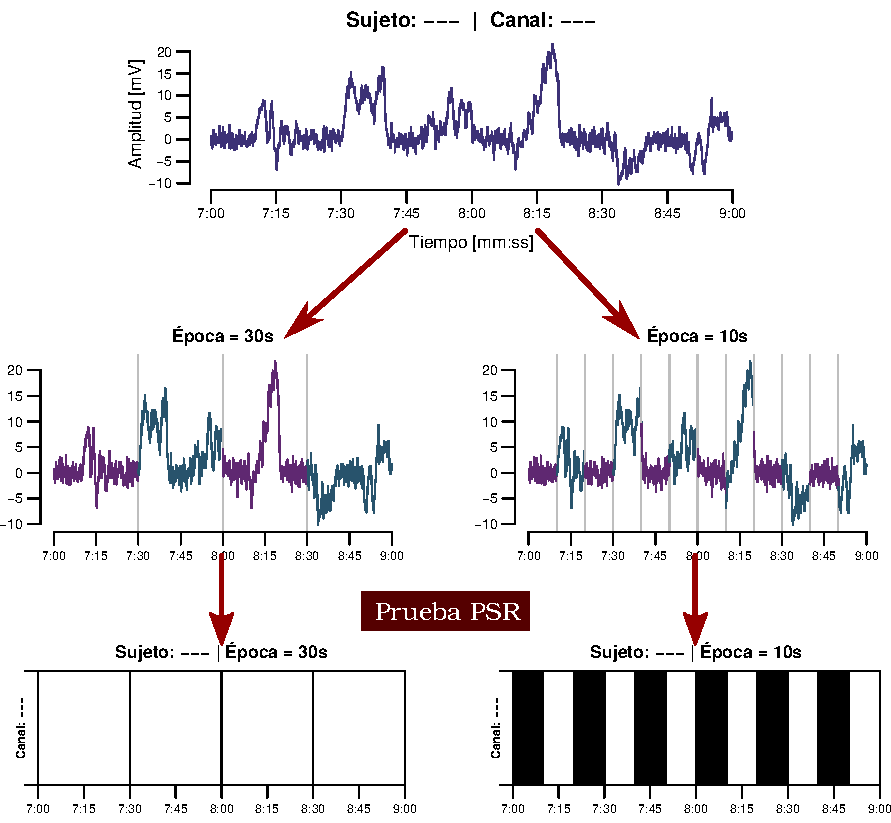
\includegraphics[width=\linewidth]{./img_diagramas/epocas_diferentes_v2.pdf}
\caption{Esquema de cómo se tomaron diferentes tamaños de época para estudiar los registros de 
PSG}
\label{epocas_diferentes}
\end{figure}

%%%%%%%%%%%%%%%%%%%%%%%%%%%%%%%%%%%%%%%%%%%%%%%%%%%%%%%%%%%%%%%%%%%%%%%%%%%%%%%%%%%%%%%%%%%%%%%%%%%
%%%%%%%%%%%%%%%%%%%%%%%%%%%%%%%%%%%%%%%%%%%%%%%%%%%%%%%%%%%%%%%%%%%%%%%%%%%%%%%%%%%%%%%%%%%%%%%%%%%
%%%%%%%%%%%%%%%%%%%%%%%%%%%%%%%%%%%%%%%%%%%%%%%%%%%%%%%%%%%%%%%%%%%%%%%%%%%%%%%%%%%%%%%%%%%%%%%%%%%
%%%%%%%%%%%%%%%%%%%%%%%%%%%%%%%%%%%%%%%%%%%%%%%%%%%%%%%%%%%%%%%%%%%%%%%%%%%%%%%%%%%%%%%%%%%%%%%%%%%
